\documentclass[14pt]{extarticle}

\usepackage[margin=0.5in]{geometry}
\usepackage{amsmath}
\usepackage[none]{hyphenat}
\usepackage{pgfplots}
\usepackage{amssymb}
\usepackage{amsmath}
\usepackage{multicol}
\usepackage{tikz}
\usepackage{tikz-3dplot}
\usetikzlibrary{angles, quotes}

\pgfplotsset{compat=newest}

\title{EE-220 Homework 12}
\author{Jonathan Forhan}
\date{ }

\renewcommand{\thesubsection}{\thesection-\alph{subsection}}

\begin{document}

\maketitle

\boldmath
\section{Given the magnetic field $\vec{H}=3y^2\vec{a}_x$, find the
  current passing through a square in the \textit{x-y} plane
  that has one corner at the origin and the opposite
  corner at $(2,2,0)$.}
\unboldmath

\begin{center}
	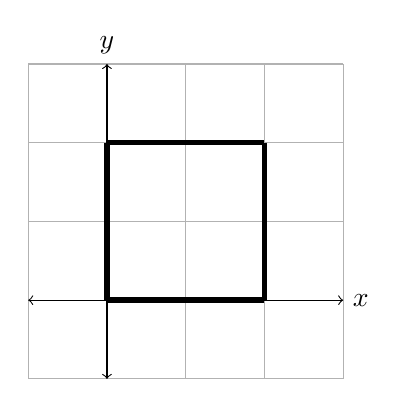
\begin{tikzpicture}
		\draw[thin,gray!60] (-2,-2) grid (2,2);
		\draw[<->] (-2,-1)--(2,-1) node[right]{$x$};
		\draw[<->] (-1,-2)--(-1,2) node[above]{$y$};
		\draw[line width=2pt,black](-1,-1)--(-1,1);
		\draw[line width=2pt,black](-1,1)--(1,1);
		\draw[line width=2pt,black](1,1)--(1,-1);
		\draw[line width=2pt,black](1,-1)--(-1,-1);
	\end{tikzpicture}
\end{center}

$$I_{\mathrm{enc}}=\oint\vec{H}\cdot\vec{dL}$$

\begin{align*}
	I_{\mathrm{enc}} & =
	\int^{2}_{0}\vec{H}\cdot\vec{dx}+
	\int^{0}_{2}\vec{H}\cdot\vec{dx}+
	\int^{2}_{0}\vec{H}\cdot\vec{dy}+
	\int^{0}_{2}\vec{H}\cdot\vec{dy}                                   \\
	0                & = \vec{H}\cdot\vec{dy}                          \\
	I_{\mathrm{enc}} & =
	\int^{2}_{0}\vec{H}\cdot\vec{dx}+ \int^{0}_{2}\vec{H}\cdot\vec{dx} \\
	I_{\mathrm{enc}} & =
	\int^{2}_{0}3(0)^2dx+ \int^{0}_{2}3(2)^2dx                         \\
	I_{\mathrm{enc}} & = 12x\bigg{|}^0_2                               \\
	I_{\mathrm{enc}} & = -24\mathrm{A}
\end{align*}

\boldmath
\section{Find the curl $\vec{\nabla}\times\vec{A}$ for the following vectors:}
\unboldmath

\boldmath
\subsection{$\vec{A}=\frac{3xy^2}{z}\vec{a}_x$}
\unboldmath

\[
	\vec{\nabla}\times\vec{A}=
	\left(\frac{\partial A_z}{\partial y}-\frac{\partial A_y}{\partial z}\right)\vec{a}_x+
	\left(\frac{\partial A_x}{\partial z}-\frac{\partial A_z}{\partial x}\right)\vec{a}_y+
	\left(\frac{\partial A_y}{\partial x}-\frac{\partial A_x}{\partial y}\right)\vec{a}_z
\]

\begin{align*}
	\vec{B} & =
	\frac{\partial A_x}{\partial z}\vec{a}_y-
	\frac{\partial A_x}{\partial y}\vec{a}_z \\
	\vec{B} & =
	-\frac{3xy^2}{z^2}\vec{a}_y-\frac{6xy}{z}\vec{a}_z
\end{align*}

\boldmath
\subsection{$\vec{A}=\rho\sin^2(\phi)\vec{a}_\rho-\rho^2z\cos(\phi)\vec{a}_\phi$}
\unboldmath

\[
	\vec{\nabla}\times\vec{A}=
	\left(\frac1\rho\frac{\partial A_z}{\partial \phi}-\frac{\partial A_\phi}{\partial z}\right)\vec{a}_\rho+
	\left(\frac{\partial A_\rho}{\partial z}-\frac{\partial A_z}{\partial \rho}\right)\vec{a}_\phi+
	\frac1\rho\left(\frac{\partial (\rho A_\phi)}{\partial \rho}-\frac{\partial A_\rho}{\partial \phi}\right)\vec{a}_z
\]

\begin{align*}
	\vec{B} & =
	\left(-\frac{\partial A_\phi}{\partial z}\right)\vec{a}_\rho+
	\left(\frac{\partial A_\rho}{\partial z}\right)\vec{a}_\phi+
	\frac1\rho\left(\frac{\partial (\rho A_\phi)}{\partial \rho}-\frac{\partial A_\rho}{\partial \phi}\right)\vec{a}_z \\
	\vec{B} & =
	\left(\rho^2\cos{\phi}\right)\vec{a}_\rho+
	(0)\vec{a}_\phi+
	\frac1\rho\left(-3\rho^2z\cos{\phi}-2\rho\sin\phi\cos\phi\right)\vec{a}_z                                          \\
	\vec{B} & =
	\left(\rho^2\cos{\phi}\right)\vec{a}_\rho-
	\left(3\rho z\cos{\phi}+2\sin\phi\cos\phi\right)\vec{a}_z
\end{align*}

\boldmath
\subsection{$\vec{A}=r^2\sin(\theta)\vec{a}_r+\frac{r}{\cos(\phi)}\vec{a}_\theta$}
\unboldmath

\[
	\vec{\nabla}\times\vec{A}=
	\frac{1}{r\sin{\theta}}\left(\frac{\partial (A_\phi\sin{\theta})}{\partial \theta}-\frac{\partial A_\theta}{\partial \phi}\right)\vec{a}_r+
	\frac1r\left(\frac{1}{\sin{\theta}}\frac{\partial A_r}{\partial \phi}-\frac{\partial (rA_\phi)}{\partial r}\right)\vec{a}_\theta+
	\frac1r\left(\frac{\partial (rA_\theta)}{\partial r}-\frac{\partial A_r}{\partial \theta}\right)\vec{a}_\phi
\]

\begin{align*}
	\vec{B} & =
	\frac{1}{r\sin{\theta}}\left(-\frac{\partial A_\theta}{\partial \phi}\right)\vec{a}_r+
	\frac1r\left(\frac{\partial (rA_\theta)}{\partial r}-\frac{\partial A_r}{\partial \theta}\right)\vec{a}_\phi \\
	\vec{B} & =
	\frac{1}{r\sin{\theta}}\left(r\tan{\phi}\sec{\phi}\right)\vec{a}_r+
	\frac1r\left(\frac{2r}{\cos{\phi}}-r^2\cos{\theta}\right)\vec{a}_\phi                                        \\
	\vec{B} & =
	\frac{\tan{\phi}\sec{\phi}}{\sin{\theta}}\vec{a}_r+
	\left(\frac{2}{\cos{\phi}}-r\cos{\theta}\right)\vec{a}_\phi                                                  \\
\end{align*}

\boldmath
\section{Suppose 2.0A current flows through 80 turns of
  a toroid that has a core cross sectional area of
  2.0cm$^2$ and a mean radius of 80cm. The core is
  99.8\% pure iron with $\mu_r=5000$. Remember that
  $\mu_0=4\pi\times 10^{-7}\mathrm{\left[\frac{H}{m}\right]}$.}
\unboldmath

\boldmath
\subsection{Calculate the magnetic flux in the toroid.}
\unboldmath

$$\phi = \frac{\mu NI}{2\pi\rho}\cdot A$$

\begin{align*}
	\phi & =
	\frac
	{(5000\cdot4\pi\times10^{-7})\cdot80\cdot2}
	{2\pi\cdot80\times10^{-2}}
	\cdot 2\times10^{-4}                            \\
	\phi & = 4\times10^{-5}\left[\mathrm{Wb}\right]
\end{align*}

\boldmath
\subsection{Calculate the energy stored in the magnetic field contained
	by the toroid.}
\unboldmath

$$W_m=\frac12LI^2$$

\begin{align*}
	L & =\frac{N\phi}{I}                 \\
	L & =\frac{80\cdot4\times10^{-5}}{2} \\
	L & = 1.6\left[\mathrm{mH}\right]
\end{align*}

$$W_m=\frac12\cdot1.6\times10^{-3}\cdot2^2=3.2\left[\mathrm{mJ}\right]$$

\end{document}
